% Created by tikzDevice version 0.12.4 on 2023-05-26 15:36:19
% !TEX encoding = UTF-8 Unicode
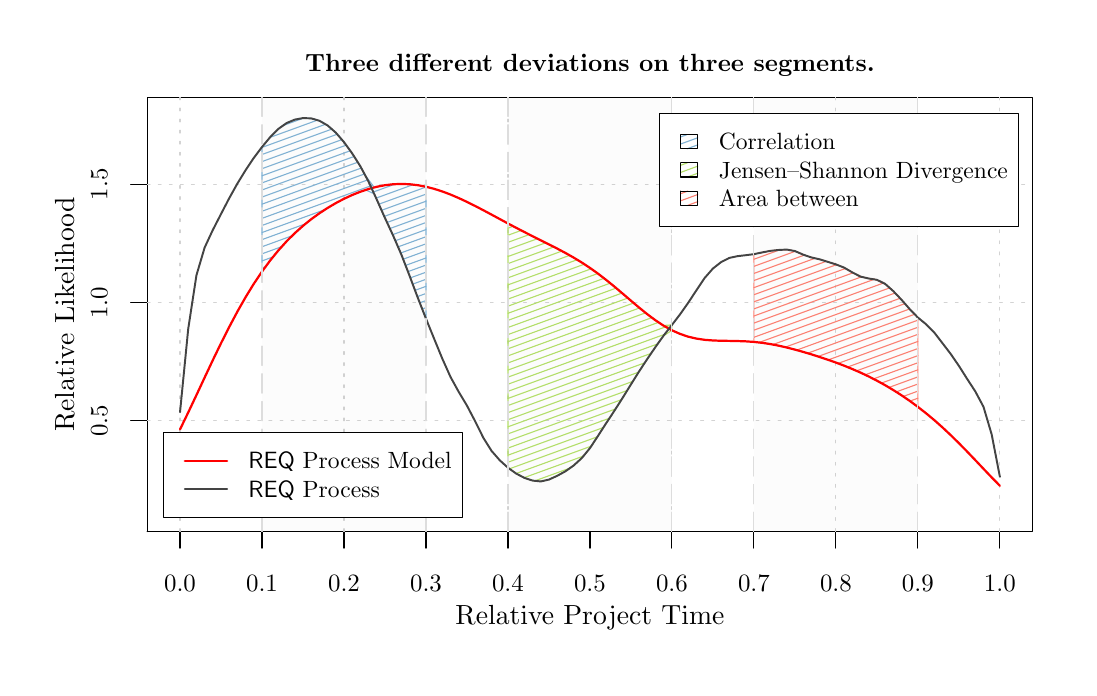
\begin{tikzpicture}[x=1pt,y=1pt]
\definecolor{fillColor}{RGB}{255,255,255}
\path[use as bounding box,fill=fillColor,fill opacity=0.00] (0,0) rectangle (376.36,231.26);
\begin{scope}
\path[clip] (  0.00,  0.00) rectangle (376.36,231.26);
\definecolor{drawColor}{RGB}{0,0,0}

\node[text=drawColor,anchor=base,inner sep=0pt, outer sep=0pt, scale=  0.90] at (203.18,215.56) {\bfseries Three different deviations on three segments.};
\end{scope}
\begin{scope}
\path[clip] (  0.00,  0.00) rectangle (376.36,231.26);
\definecolor{drawColor}{RGB}{0,0,0}

\path[draw=drawColor,line width= 0.4pt,line join=round,line cap=round] ( 55.05, 49.20) -- (351.31, 49.20);

\path[draw=drawColor,line width= 0.4pt,line join=round,line cap=round] ( 55.05, 49.20) -- ( 55.05, 43.20);

\path[draw=drawColor,line width= 0.4pt,line join=round,line cap=round] ( 84.68, 49.20) -- ( 84.68, 43.20);

\path[draw=drawColor,line width= 0.4pt,line join=round,line cap=round] (114.30, 49.20) -- (114.30, 43.20);

\path[draw=drawColor,line width= 0.4pt,line join=round,line cap=round] (143.93, 49.20) -- (143.93, 43.20);

\path[draw=drawColor,line width= 0.4pt,line join=round,line cap=round] (173.55, 49.20) -- (173.55, 43.20);

\path[draw=drawColor,line width= 0.4pt,line join=round,line cap=round] (203.18, 49.20) -- (203.18, 43.20);

\path[draw=drawColor,line width= 0.4pt,line join=round,line cap=round] (232.80, 49.20) -- (232.80, 43.20);

\path[draw=drawColor,line width= 0.4pt,line join=round,line cap=round] (262.43, 49.20) -- (262.43, 43.20);

\path[draw=drawColor,line width= 0.4pt,line join=round,line cap=round] (292.06, 49.20) -- (292.06, 43.20);

\path[draw=drawColor,line width= 0.4pt,line join=round,line cap=round] (321.68, 49.20) -- (321.68, 43.20);

\path[draw=drawColor,line width= 0.4pt,line join=round,line cap=round] (351.31, 49.20) -- (351.31, 43.20);

\node[text=drawColor,anchor=base,inner sep=0pt, outer sep=0pt, scale=  0.90] at ( 55.05, 27.60) {0.0};

\node[text=drawColor,anchor=base,inner sep=0pt, outer sep=0pt, scale=  0.90] at ( 84.68, 27.60) {0.1};

\node[text=drawColor,anchor=base,inner sep=0pt, outer sep=0pt, scale=  0.90] at (114.30, 27.60) {0.2};

\node[text=drawColor,anchor=base,inner sep=0pt, outer sep=0pt, scale=  0.90] at (143.93, 27.60) {0.3};

\node[text=drawColor,anchor=base,inner sep=0pt, outer sep=0pt, scale=  0.90] at (173.55, 27.60) {0.4};

\node[text=drawColor,anchor=base,inner sep=0pt, outer sep=0pt, scale=  0.90] at (203.18, 27.60) {0.5};

\node[text=drawColor,anchor=base,inner sep=0pt, outer sep=0pt, scale=  0.90] at (232.80, 27.60) {0.6};

\node[text=drawColor,anchor=base,inner sep=0pt, outer sep=0pt, scale=  0.90] at (262.43, 27.60) {0.7};

\node[text=drawColor,anchor=base,inner sep=0pt, outer sep=0pt, scale=  0.90] at (292.06, 27.60) {0.8};

\node[text=drawColor,anchor=base,inner sep=0pt, outer sep=0pt, scale=  0.90] at (321.68, 27.60) {0.9};

\node[text=drawColor,anchor=base,inner sep=0pt, outer sep=0pt, scale=  0.90] at (351.31, 27.60) {1.0};

\path[draw=drawColor,line width= 0.4pt,line join=round,line cap=round] ( 43.20, 89.18) -- ( 43.20,174.62);

\path[draw=drawColor,line width= 0.4pt,line join=round,line cap=round] ( 43.20, 89.18) -- ( 37.20, 89.18);

\path[draw=drawColor,line width= 0.4pt,line join=round,line cap=round] ( 43.20,131.90) -- ( 37.20,131.90);

\path[draw=drawColor,line width= 0.4pt,line join=round,line cap=round] ( 43.20,174.62) -- ( 37.20,174.62);

\node[text=drawColor,rotate= 90.00,anchor=base,inner sep=0pt, outer sep=0pt, scale=  0.90] at ( 28.80, 89.18) {0.5};

\node[text=drawColor,rotate= 90.00,anchor=base,inner sep=0pt, outer sep=0pt, scale=  0.90] at ( 28.80,131.90) {1.0};

\node[text=drawColor,rotate= 90.00,anchor=base,inner sep=0pt, outer sep=0pt, scale=  0.90] at ( 28.80,174.62) {1.5};

\node[text=drawColor,anchor=base,inner sep=0pt, outer sep=0pt, scale=  1.00] at (203.18, 15.60) {Relative Project Time};

\node[text=drawColor,rotate= 90.00,anchor=base,inner sep=0pt, outer sep=0pt, scale=  1.00] at ( 16.80,127.63) {Relative Likelihood};

\path[draw=drawColor,line width= 0.4pt,line join=round,line cap=round] ( 43.20, 49.20) --
	(363.16, 49.20) --
	(363.16,206.06) --
	( 43.20,206.06) --
	( 43.20, 49.20);
\end{scope}
\begin{scope}
\path[clip] ( 43.20, 49.20) rectangle (363.16,206.06);
\definecolor{drawColor}{RGB}{211,211,211}

\path[draw=drawColor,line width= 0.4pt,dash pattern=on 1pt off 3pt ,line join=round,line cap=round] ( 55.05, 49.20) -- ( 55.05,206.06);

\path[draw=drawColor,line width= 0.4pt,dash pattern=on 1pt off 3pt ,line join=round,line cap=round] (114.30, 49.20) -- (114.30,206.06);

\path[draw=drawColor,line width= 0.4pt,dash pattern=on 1pt off 3pt ,line join=round,line cap=round] (173.55, 49.20) -- (173.55,206.06);

\path[draw=drawColor,line width= 0.4pt,dash pattern=on 1pt off 3pt ,line join=round,line cap=round] (232.80, 49.20) -- (232.80,206.06);

\path[draw=drawColor,line width= 0.4pt,dash pattern=on 1pt off 3pt ,line join=round,line cap=round] (292.06, 49.20) -- (292.06,206.06);

\path[draw=drawColor,line width= 0.4pt,dash pattern=on 1pt off 3pt ,line join=round,line cap=round] (351.31, 49.20) -- (351.31,206.06);

\path[draw=drawColor,line width= 0.4pt,dash pattern=on 1pt off 3pt ,line join=round,line cap=round] ( 43.20, 89.18) -- (363.16, 89.18);

\path[draw=drawColor,line width= 0.4pt,dash pattern=on 1pt off 3pt ,line join=round,line cap=round] ( 43.20,131.90) -- (363.16,131.90);

\path[draw=drawColor,line width= 0.4pt,dash pattern=on 1pt off 3pt ,line join=round,line cap=round] ( 43.20,174.62) -- (363.16,174.62);
\definecolor{fillColor}{RGB}{0,0,0}

\path[fill=fillColor,fill opacity=0.01] (262.43, 46.47) rectangle (321.68,302.78);
\definecolor{drawColor}{RGB}{251,128,114}

\path[draw=drawColor,line width= 0.4pt,line join=round,line cap=round] (321.16, 94.61) -- (321.68, 94.80);

\path[draw=drawColor,line width= 0.4pt,line join=round,line cap=round] (318.81, 96.32) -- (321.68, 97.37);

\path[draw=drawColor,line width= 0.4pt,line join=round,line cap=round] (316.37, 98.00) -- (321.68, 99.93);

\path[draw=drawColor,line width= 0.4pt,line join=round,line cap=round] (313.84, 99.64) -- (321.68,102.49);

\path[draw=drawColor,line width= 0.4pt,line join=round,line cap=round] (311.21,101.25) -- (321.68,105.06);

\path[draw=drawColor,line width= 0.4pt,line join=round,line cap=round] (308.48,102.82) -- (321.68,107.62);

\path[draw=drawColor,line width= 0.4pt,line join=round,line cap=round] (305.63,104.34) -- (321.68,110.18);

\path[draw=drawColor,line width= 0.4pt,line join=round,line cap=round] (302.65,105.82) -- (321.68,112.75);

\path[draw=drawColor,line width= 0.4pt,line join=round,line cap=round] (299.52,107.25) -- (321.68,115.31);

\path[draw=drawColor,line width= 0.4pt,line join=round,line cap=round] (296.25,108.62) -- (321.68,117.88);

\path[draw=drawColor,line width= 0.4pt,line join=round,line cap=round] (292.84,109.94) -- (321.68,120.44);

\path[draw=drawColor,line width= 0.4pt,line join=round,line cap=round] (289.29,111.21) -- (321.68,123.00);

\path[draw=drawColor,line width= 0.4pt,line join=round,line cap=round] (285.61,112.44) -- (321.68,125.57);

\path[draw=drawColor,line width= 0.4pt,line join=round,line cap=round] (281.82,113.62) -- (320.52,127.71);

\path[draw=drawColor,line width= 0.4pt,line join=round,line cap=round] (277.89,114.75) -- (318.69,129.61);

\path[draw=drawColor,line width= 0.4pt,line join=round,line cap=round] (273.74,115.81) -- (316.97,131.54);

\path[draw=drawColor,line width= 0.4pt,line join=round,line cap=round] (269.29,116.75) -- (315.25,133.48);

\path[draw=drawColor,line width= 0.4pt,line join=round,line cap=round] (264.29,117.50) -- (313.43,135.38);

\path[draw=drawColor,line width= 0.4pt,line join=round,line cap=round] (262.43,119.38) -- (311.48,137.23);

\path[draw=drawColor,line width= 0.4pt,line join=round,line cap=round] (262.43,121.95) -- (309.33,139.02);

\path[draw=drawColor,line width= 0.4pt,line join=round,line cap=round] (262.43,124.51) -- (305.94,140.35);

\path[draw=drawColor,line width= 0.4pt,line join=round,line cap=round] (262.43,127.07) -- (301.43,141.27);

\path[draw=drawColor,line width= 0.4pt,line join=round,line cap=round] (262.43,129.64) -- (298.29,142.69);

\path[draw=drawColor,line width= 0.4pt,line join=round,line cap=round] (262.43,132.20) -- (295.48,144.23);

\path[draw=drawColor,line width= 0.4pt,line join=round,line cap=round] (262.43,134.76) -- (292.26,145.62);

\path[draw=drawColor,line width= 0.4pt,line join=round,line cap=round] (262.43,137.33) -- (288.54,146.83);

\path[draw=drawColor,line width= 0.4pt,line join=round,line cap=round] (262.43,139.89) -- (284.51,147.93);

\path[draw=drawColor,line width= 0.4pt,line join=round,line cap=round] (262.43,142.45) -- (280.64,149.08);

\path[draw=drawColor,line width= 0.4pt,line join=round,line cap=round] (262.43,145.02) -- (277.30,150.43);

\path[draw=drawColor,line width= 0.4pt,line join=round,line cap=round] (262.43,147.58) -- (271.71,150.96);

\path[draw=drawColor,line width= 0.4pt,line join=round,line cap=round] (262.43,149.42) --
	(265.55,150.08) --
	(268.67,150.65) --
	(271.79,150.97) --
	(274.90,151.05) --
	(278.02,150.24) --
	(281.14,148.86) --
	(284.26,147.99) --
	(287.38,147.21) --
	(290.50,146.20) --
	(293.62,145.18) --
	(296.73,143.59) --
	(299.85,141.79) --
	(302.97,140.76) --
	(306.09,140.32) --
	(309.21,139.11) --
	(312.33,136.53) --
	(315.44,133.28) --
	(318.56,129.74) --
	(321.68,126.50) --
	(321.68, 94.23) --
	(318.56, 96.51) --
	(315.44, 98.63) --
	(312.33,100.60) --
	(309.21,102.42) --
	(306.09,104.11) --
	(302.97,105.67) --
	(299.85,107.11) --
	(296.73,108.43) --
	(293.62,109.66) --
	(290.50,110.80) --
	(287.38,111.87) --
	(284.26,112.88) --
	(281.14,113.83) --
	(278.02,114.72) --
	(274.90,115.54) --
	(271.79,116.26) --
	(268.67,116.87) --
	(265.55,117.36) --
	(262.43,117.70) --
	(262.43,149.42);

\path[fill=fillColor,fill opacity=0.01] ( 84.68, 46.47) rectangle (143.93,302.78);
\definecolor{drawColor}{RGB}{128,177,211}

\path[draw=drawColor,line width= 0.4pt,line join=round,line cap=round] (143.44,127.35) -- (143.93,127.52);

\path[draw=drawColor,line width= 0.4pt,line join=round,line cap=round] (142.57,129.59) -- (143.93,130.09);

\path[draw=drawColor,line width= 0.4pt,line join=round,line cap=round] (141.69,131.84) -- (143.93,132.65);

\path[draw=drawColor,line width= 0.4pt,line join=round,line cap=round] (140.82,134.08) -- (143.93,135.21);

\path[draw=drawColor,line width= 0.4pt,line join=round,line cap=round] (139.97,136.34) -- (143.93,137.78);

\path[draw=drawColor,line width= 0.4pt,line join=round,line cap=round] (139.13,138.59) -- (143.93,140.34);

\path[draw=drawColor,line width= 0.4pt,line join=round,line cap=round] (138.28,140.85) -- (143.93,142.90);

\path[draw=drawColor,line width= 0.4pt,line join=round,line cap=round] (137.42,143.10) -- (143.93,145.47);

\path[draw=drawColor,line width= 0.4pt,line join=round,line cap=round] (136.55,145.35) -- (143.93,148.03);

\path[draw=drawColor,line width= 0.4pt,line join=round,line cap=round] (135.67,147.59) -- (143.93,150.60);

\path[draw=drawColor,line width= 0.4pt,line join=round,line cap=round] (134.79,149.83) -- (143.93,153.16);

\path[draw=drawColor,line width= 0.4pt,line join=round,line cap=round] (133.84,152.05) -- (143.93,155.72);

\path[draw=drawColor,line width= 0.4pt,line join=round,line cap=round] (132.86,154.26) -- (143.93,158.29);

\path[draw=drawColor,line width= 0.4pt,line join=round,line cap=round] (131.88,156.46) -- (143.93,160.85);

\path[draw=drawColor,line width= 0.4pt,line join=round,line cap=round] (130.88,158.67) -- (143.93,163.41);

\path[draw=drawColor,line width= 0.4pt,line join=round,line cap=round] ( 84.68,144.41) -- ( 85.97,144.88);

\path[draw=drawColor,line width= 0.4pt,line join=round,line cap=round] (129.87,160.86) -- (143.93,165.98);

\path[draw=drawColor,line width= 0.4pt,line join=round,line cap=round] ( 84.68,146.98) -- ( 88.69,148.43);

\path[draw=drawColor,line width= 0.4pt,line join=round,line cap=round] (128.86,163.06) -- (143.93,168.54);

\path[draw=drawColor,line width= 0.4pt,line join=round,line cap=round] ( 84.68,149.54) -- ( 91.82,152.14);

\path[draw=drawColor,line width= 0.4pt,line join=round,line cap=round] (127.87,165.26) -- (143.93,171.10);

\path[draw=drawColor,line width= 0.4pt,line join=round,line cap=round] ( 84.68,152.10) -- ( 95.60,156.08);

\path[draw=drawColor,line width= 0.4pt,line join=round,line cap=round] (126.89,167.47) -- (143.93,173.67);

\path[draw=drawColor,line width= 0.4pt,line join=round,line cap=round] ( 84.68,154.67) -- (100.36,160.37);

\path[draw=drawColor,line width= 0.4pt,line join=round,line cap=round] (125.91,169.67) -- (139.26,174.53);

\path[draw=drawColor,line width= 0.4pt,line join=round,line cap=round] ( 84.68,157.23) -- (107.48,165.53);

\path[draw=drawColor,line width= 0.4pt,line join=round,line cap=round] (124.30,171.65) -- (132.65,174.69);

\path[draw=drawColor,line width= 0.4pt,line join=round,line cap=round] ( 84.68,159.79) -- (124.63,174.33);

\path[draw=drawColor,line width= 0.4pt,line join=round,line cap=round] ( 84.68,162.36) -- (123.13,176.35);

\path[draw=drawColor,line width= 0.4pt,line join=round,line cap=round] ( 84.68,164.92) -- (121.73,178.41);

\path[draw=drawColor,line width= 0.4pt,line join=round,line cap=round] ( 84.68,167.48) -- (120.51,180.53);

\path[draw=drawColor,line width= 0.4pt,line join=round,line cap=round] ( 84.68,170.05) -- (119.30,182.65);

\path[draw=drawColor,line width= 0.4pt,line join=round,line cap=round] ( 84.68,172.61) -- (117.95,184.72);

\path[draw=drawColor,line width= 0.4pt,line join=round,line cap=round] ( 84.68,175.17) -- (116.57,186.78);

\path[draw=drawColor,line width= 0.4pt,line join=round,line cap=round] ( 84.68,177.74) -- (115.09,188.81);

\path[draw=drawColor,line width= 0.4pt,line join=round,line cap=round] ( 84.68,180.30) -- (113.53,190.80);

\path[draw=drawColor,line width= 0.4pt,line join=round,line cap=round] ( 84.68,182.87) -- (111.81,192.74);

\path[draw=drawColor,line width= 0.4pt,line join=round,line cap=round] ( 84.68,185.43) -- (109.94,194.62);

\path[draw=drawColor,line width= 0.4pt,line join=round,line cap=round] ( 84.68,187.99) -- (107.60,196.34);

\path[draw=drawColor,line width= 0.4pt,line join=round,line cap=round] ( 87.57,191.61) -- (104.63,197.82);

\path[draw=drawColor,line width= 0.4pt,line join=round,line cap=round] ( 92.35,195.91) -- ( 99.55,198.53);

\path[draw=drawColor,line width= 0.4pt,line join=round,line cap=round] ( 84.68,188.16) --
	( 87.79,191.88) --
	( 90.91,194.95) --
	( 94.03,197.04) --
	( 97.15,198.21) --
	(100.27,198.63) --
	(103.39,198.30) --
	(106.51,197.10) --
	(109.62,194.94) --
	(112.74,191.80) --
	(115.86,187.83) --
	(118.98,183.20) --
	(122.10,177.76) --
	(125.22,173.54) --
	(128.33,174.21) --
	(131.45,174.63) --
	(134.57,174.79) --
	(137.69,174.71) --
	(140.81,174.36) --
	(143.93,173.78) --
	(143.93,126.10) --
	(140.81,134.11) --
	(137.69,142.42) --
	(134.57,150.39) --
	(131.45,157.43) --
	(128.33,164.20) --
	(125.22,171.24) --
	(122.10,172.63) --
	(118.98,171.50) --
	(115.86,170.16) --
	(112.74,168.62) --
	(109.62,166.87) --
	(106.51,164.92) --
	(103.39,162.74) --
	(100.27,160.30) --
	( 97.15,157.59) --
	( 94.03,154.55) --
	( 90.91,151.15) --
	( 87.79,147.35) --
	( 84.68,143.13) --
	( 84.68,188.16);

\path[fill=fillColor,fill opacity=0.01] (173.55, 46.47) rectangle (232.80,302.78);
\definecolor{drawColor}{RGB}{179,222,105}

\path[draw=drawColor,line width= 0.4pt,line join=round,line cap=round] (183.24, 67.49) -- (196.03, 72.14);

\path[draw=drawColor,line width= 0.4pt,line join=round,line cap=round] (179.39, 68.65) -- (200.79, 76.44);

\path[draw=drawColor,line width= 0.4pt,line join=round,line cap=round] (176.50, 70.16) -- (203.57, 80.02);

\path[draw=drawColor,line width= 0.4pt,line join=round,line cap=round] (174.11, 71.86) -- (205.87, 83.42);

\path[draw=drawColor,line width= 0.4pt,line join=round,line cap=round] (173.55, 74.22) -- (208.01, 86.76);

\path[draw=drawColor,line width= 0.4pt,line join=round,line cap=round] (173.55, 76.78) -- (210.23, 90.13);

\path[draw=drawColor,line width= 0.4pt,line join=round,line cap=round] (173.55, 79.34) -- (212.42, 93.49);

\path[draw=drawColor,line width= 0.4pt,line join=round,line cap=round] (173.55, 81.91) -- (214.57, 96.84);

\path[draw=drawColor,line width= 0.4pt,line join=round,line cap=round] (173.55, 84.47) -- (216.63,100.15);

\path[draw=drawColor,line width= 0.4pt,line join=round,line cap=round] (173.55, 87.03) -- (218.69,103.46);

\path[draw=drawColor,line width= 0.4pt,line join=round,line cap=round] (173.55, 89.60) -- (220.78,106.79);

\path[draw=drawColor,line width= 0.4pt,line join=round,line cap=round] (173.55, 92.16) -- (222.97,110.15);

\path[draw=drawColor,line width= 0.4pt,line join=round,line cap=round] (173.55, 94.72) -- (225.26,113.55);

\path[draw=drawColor,line width= 0.4pt,line join=round,line cap=round] (173.55, 97.29) -- (227.65,116.98);

\path[draw=drawColor,line width= 0.4pt,line join=round,line cap=round] (173.55, 99.85) -- (231.18,120.82);

\path[draw=drawColor,line width= 0.4pt,line join=round,line cap=round] (173.55,102.42) -- (232.38,123.83);

\path[draw=drawColor,line width= 0.4pt,line join=round,line cap=round] (173.55,104.98) -- (227.98,124.79);

\path[draw=drawColor,line width= 0.4pt,line join=round,line cap=round] (173.55,107.54) -- (225.57,126.48);

\path[draw=drawColor,line width= 0.4pt,line join=round,line cap=round] (173.55,110.11) -- (223.28,128.21);

\path[draw=drawColor,line width= 0.4pt,line join=round,line cap=round] (173.55,112.67) -- (221.11,129.98);

\path[draw=drawColor,line width= 0.4pt,line join=round,line cap=round] (173.55,115.23) -- (218.98,131.77);

\path[draw=drawColor,line width= 0.4pt,line join=round,line cap=round] (173.55,117.80) -- (216.87,133.56);

\path[draw=drawColor,line width= 0.4pt,line join=round,line cap=round] (173.55,120.36) -- (214.77,135.36);

\path[draw=drawColor,line width= 0.4pt,line join=round,line cap=round] (173.55,122.92) -- (212.64,137.15);

\path[draw=drawColor,line width= 0.4pt,line join=round,line cap=round] (173.55,125.49) -- (210.49,138.93);

\path[draw=drawColor,line width= 0.4pt,line join=round,line cap=round] (173.55,128.05) -- (208.29,140.69);

\path[draw=drawColor,line width= 0.4pt,line join=round,line cap=round] (173.55,130.62) -- (206.00,142.42);

\path[draw=drawColor,line width= 0.4pt,line join=round,line cap=round] (173.55,133.18) -- (203.62,144.12);

\path[draw=drawColor,line width= 0.4pt,line join=round,line cap=round] (173.55,135.74) -- (201.16,145.79);

\path[draw=drawColor,line width= 0.4pt,line join=round,line cap=round] (173.55,138.31) -- (198.58,147.41);

\path[draw=drawColor,line width= 0.4pt,line join=round,line cap=round] (173.55,140.87) -- (195.86,148.99);

\path[draw=drawColor,line width= 0.4pt,line join=round,line cap=round] (173.55,143.43) -- (193.05,150.53);

\path[draw=drawColor,line width= 0.4pt,line join=round,line cap=round] (173.55,146.00) -- (190.15,152.04);

\path[draw=drawColor,line width= 0.4pt,line join=round,line cap=round] (173.55,148.56) -- (187.20,153.53);

\path[draw=drawColor,line width= 0.4pt,line join=round,line cap=round] (173.55,151.12) -- (184.23,155.01);

\path[draw=drawColor,line width= 0.4pt,line join=round,line cap=round] (173.55,153.69) -- (181.27,156.50);

\path[draw=drawColor,line width= 0.4pt,line join=round,line cap=round] (173.55,156.25) -- (178.35,158.00);

\path[draw=drawColor,line width= 0.4pt,line join=round,line cap=round] (173.55,158.81) -- (175.45,159.51);

\path[draw=drawColor,line width= 0.4pt,line join=round,line cap=round] (173.55,160.51) --
	(176.67,158.86) --
	(179.79,157.25) --
	(182.91,155.67) --
	(186.03,154.11) --
	(189.15,152.55) --
	(192.26,150.95) --
	(195.38,149.27) --
	(198.50,147.46) --
	(201.62,145.50) --
	(204.74,143.36) --
	(207.86,141.04) --
	(210.98,138.55) --
	(214.09,135.94) --
	(217.21,133.27) --
	(220.33,130.62) --
	(223.45,128.07) --
	(226.57,125.72) --
	(229.69,123.65) --
	(232.80,123.85) --
	(232.80,121.90) --
	(229.69,119.84) --
	(226.57,115.46) --
	(223.45,110.88) --
	(220.33,106.10) --
	(217.21,101.09) --
	(214.09, 96.07) --
	(210.98, 91.26) --
	(207.86, 86.52) --
	(204.74, 81.64) --
	(201.62, 77.30) --
	(198.50, 74.08) --
	(195.38, 71.63) --
	(192.26, 69.80) --
	(189.15, 68.27) --
	(186.03, 67.35) --
	(182.91, 67.50) --
	(179.79, 68.45) --
	(176.67, 70.04) --
	(173.55, 72.25) --
	(173.55,160.51);
\definecolor{drawColor}{RGB}{255,0,0}

\path[draw=drawColor,line width= 0.8pt,line join=round,line cap=round] ( 55.05, 86.09) --
	( 58.01, 92.21) --
	( 60.98, 98.49) --
	( 63.94,104.83) --
	( 66.90,111.11) --
	( 69.86,117.23) --
	( 72.83,123.11) --
	( 75.79,128.68) --
	( 78.75,133.88) --
	( 81.71,138.71) --
	( 84.68,143.13) --
	( 87.64,147.15) --
	( 90.60,150.78) --
	( 93.56,154.06) --
	( 96.53,157.01) --
	( 99.49,159.65) --
	(102.45,162.04) --
	(105.41,164.18) --
	(108.38,166.12) --
	(111.34,167.86) --
	(114.30,169.42) --
	(117.26,170.79) --
	(120.23,171.98) --
	(123.19,172.97) --
	(126.15,173.76) --
	(129.11,174.34) --
	(132.08,174.68) --
	(135.04,174.80) --
	(138.00,174.68) --
	(140.96,174.34) --
	(143.93,173.78) --
	(146.89,173.02) --
	(149.85,172.07) --
	(152.82,170.95) --
	(155.78,169.68) --
	(158.74,168.30) --
	(161.70,166.83) --
	(164.67,165.28) --
	(167.63,163.70) --
	(170.59,162.10) --
	(173.55,160.51) --
	(176.52,158.94) --
	(179.48,157.41) --
	(182.44,155.91) --
	(185.40,154.43) --
	(188.37,152.94) --
	(191.33,151.44) --
	(194.29,149.87) --
	(197.25,148.20) --
	(200.22,146.40) --
	(203.18,144.45) --
	(206.14,142.34) --
	(209.10,140.06) --
	(212.07,137.65) --
	(215.03,135.14) --
	(217.99,132.60) --
	(220.95,130.10) --
	(223.92,127.71) --
	(226.88,125.50) --
	(229.84,123.55) --
	(232.80,121.90) --
	(235.77,120.58) --
	(238.73,119.59) --
	(241.69,118.90) --
	(244.65,118.46) --
	(247.62,118.23) --
	(250.58,118.12) --
	(253.54,118.08) --
	(256.51,118.02) --
	(259.47,117.91) --
	(262.43,117.70) --
	(265.39,117.38) --
	(268.36,116.93) --
	(271.32,116.36) --
	(274.28,115.69) --
	(277.24,114.93) --
	(280.21,114.10) --
	(283.17,113.22) --
	(286.13,112.28) --
	(289.09,111.29) --
	(292.06,110.24) --
	(295.02,109.12) --
	(297.98,107.91) --
	(300.94,106.62) --
	(303.91,105.22) --
	(306.87,103.70) --
	(309.83,102.07) --
	(312.79,100.31) --
	(315.76, 98.42) --
	(318.72, 96.40) --
	(321.68, 94.23) --
	(324.64, 91.91) --
	(327.61, 89.44) --
	(330.57, 86.81) --
	(333.53, 84.03) --
	(336.49, 81.12) --
	(339.46, 78.09) --
	(342.42, 74.99) --
	(345.38, 71.86) --
	(348.34, 68.75) --
	(351.31, 65.73);
\definecolor{drawColor}{RGB}{68,68,68}

\path[draw=drawColor,line width= 0.7pt,line join=round,line cap=round] ( 55.05, 92.30) --
	( 58.01,122.40) --
	( 60.98,141.78) --
	( 63.94,151.79) --
	( 66.90,158.16) --
	( 69.86,163.92) --
	( 72.83,169.64) --
	( 75.79,174.95) --
	( 78.75,179.77) --
	( 81.71,184.20) --
	( 84.68,188.16) --
	( 87.64,191.71) --
	( 90.60,194.69) --
	( 93.56,196.79) --
	( 96.53,198.04) --
	( 99.49,198.59) --
	(102.45,198.48) --
	(105.41,197.63) --
	(108.38,195.92) --
	(111.34,193.33) --
	(114.30,189.90) --
	(117.26,185.83) --
	(120.23,181.14) --
	(123.19,175.59) --
	(126.15,169.14) --
	(129.11,162.48) --
	(132.08,156.08) --
	(135.04,149.25) --
	(138.00,141.59) --
	(140.96,133.70) --
	(143.93,126.10) --
	(146.89,118.81) --
	(149.85,111.60) --
	(152.82,104.99) --
	(155.78, 99.61) --
	(158.74, 94.68) --
	(161.70, 89.01) --
	(164.67, 83.03) --
	(167.63, 78.31) --
	(170.59, 74.93) --
	(173.55, 72.25) --
	(176.52, 70.13) --
	(179.48, 68.58) --
	(182.44, 67.60) --
	(185.40, 67.29) --
	(188.37, 67.96) --
	(191.33, 69.32) --
	(194.29, 70.94) --
	(197.25, 73.02) --
	(200.22, 75.72) --
	(203.18, 79.33) --
	(206.14, 83.83) --
	(209.10, 88.44) --
	(212.07, 92.92) --
	(215.03, 97.56) --
	(217.99,102.35) --
	(220.95,107.08) --
	(223.92,111.57) --
	(226.88,115.91) --
	(229.84,120.05) --
	(232.80,123.85) --
	(235.77,127.72) --
	(238.73,131.92) --
	(241.69,136.43) --
	(244.65,140.84) --
	(247.62,144.23) --
	(250.58,146.56) --
	(253.54,148.06) --
	(256.51,148.70) --
	(259.47,149.04) --
	(262.43,149.42) --
	(265.39,150.04) --
	(268.36,150.61) --
	(271.32,150.93) --
	(274.28,151.08) --
	(277.24,150.54) --
	(280.21,149.25) --
	(283.17,148.23) --
	(286.13,147.57) --
	(289.09,146.65) --
	(292.06,145.72) --
	(295.02,144.55) --
	(297.98,142.83) --
	(300.94,141.31) --
	(303.91,140.62) --
	(306.87,140.15) --
	(309.83,138.69) --
	(312.79,136.06) --
	(315.76,132.94) --
	(318.72,129.56) --
	(321.68,126.50) --
	(324.64,124.09) --
	(327.61,121.08) --
	(330.57,117.23) --
	(333.53,113.36) --
	(336.49,109.06) --
	(339.46,104.36) --
	(342.42, 99.82) --
	(345.38, 94.26) --
	(348.34, 84.27) --
	(351.31, 68.95);
\definecolor{drawColor}{RGB}{221,221,221}

\path[draw=drawColor,line width= 0.4pt,dash pattern=on 7pt off 3pt ,line join=round,line cap=round] ( 84.68, 49.20) -- ( 84.68,206.06);

\path[draw=drawColor,line width= 0.4pt,dash pattern=on 7pt off 3pt ,line join=round,line cap=round] (143.93, 49.20) -- (143.93,206.06);

\path[draw=drawColor,line width= 0.4pt,dash pattern=on 7pt off 3pt ,line join=round,line cap=round] (173.55, 49.20) -- (173.55,206.06);

\path[draw=drawColor,line width= 0.4pt,dash pattern=on 7pt off 3pt ,line join=round,line cap=round] (232.80, 49.20) -- (232.80,206.06);

\path[draw=drawColor,line width= 0.4pt,dash pattern=on 7pt off 3pt ,line join=round,line cap=round] (262.43, 49.20) -- (262.43,206.06);

\path[draw=drawColor,line width= 0.4pt,dash pattern=on 7pt off 3pt ,line join=round,line cap=round] (321.68, 49.20) -- (321.68,206.06);
\definecolor{drawColor}{RGB}{0,0,0}
\definecolor{fillColor}{RGB}{255,255,255}

\path[draw=drawColor,line width= 0.4pt,line join=round,line cap=round,fill=fillColor] (228.36,200.25) rectangle (358.01,159.45);
\definecolor{drawColor}{RGB}{128,177,211}

\path[draw=drawColor,line width= 0.4pt,line join=round,line cap=round] (238.29,187.50) -- (242.13,188.90);

\path[draw=drawColor,line width= 0.4pt,line join=round,line cap=round] (236.01,189.24) -- (242.13,191.47);

\path[draw=drawColor,line width= 0.4pt,line join=round,line cap=round] (236.01,191.80) -- (238.21,192.60);
\definecolor{drawColor}{RGB}{179,222,105}

\path[draw=drawColor,line width= 0.4pt,line join=round,line cap=round] (238.44,177.30) -- (242.13,178.65);

\path[draw=drawColor,line width= 0.4pt,line join=round,line cap=round] (236.01,178.98) -- (242.13,181.21);

\path[draw=drawColor,line width= 0.4pt,line join=round,line cap=round] (236.01,181.55) -- (238.36,182.40);
\definecolor{drawColor}{RGB}{251,128,114}

\path[draw=drawColor,line width= 0.4pt,line join=round,line cap=round] (238.59,167.10) -- (242.13,168.39);

\path[draw=drawColor,line width= 0.4pt,line join=round,line cap=round] (236.01,168.73) -- (242.13,170.96);

\path[draw=drawColor,line width= 0.4pt,line join=round,line cap=round] (236.01,171.29) -- (238.51,172.20);
\definecolor{drawColor}{RGB}{0,0,0}

\path[draw=drawColor,line width= 0.4pt,line join=round,line cap=round] (236.01,192.60) --
	(242.13,192.60) --
	(242.13,187.50) --
	(236.01,187.50) --
	(236.01,192.60);

\path[draw=drawColor,line width= 0.4pt,line join=round,line cap=round] (236.01,182.40) --
	(242.13,182.40) --
	(242.13,177.30) --
	(236.01,177.30) --
	(236.01,182.40);

\path[draw=drawColor,line width= 0.4pt,line join=round,line cap=round] (236.01,172.20) --
	(242.13,172.20) --
	(242.13,167.10) --
	(236.01,167.10) --
	(236.01,172.20);

\node[text=drawColor,anchor=base west,inner sep=0pt, outer sep=0pt, scale=  0.85] at (249.78,187.13) {Correlation};

\node[text=drawColor,anchor=base west,inner sep=0pt, outer sep=0pt, scale=  0.85] at (249.78,176.93) {Jensen--Shannon Divergence};

\node[text=drawColor,anchor=base west,inner sep=0pt, outer sep=0pt, scale=  0.85] at (249.78,166.73) {Area between};

\path[draw=drawColor,line width= 0.4pt,line join=round,line cap=round,fill=fillColor] ( 49.13, 84.91) rectangle (157.02, 54.31);
\definecolor{drawColor}{RGB}{255,0,0}

\path[draw=drawColor,line width= 0.8pt,line join=round,line cap=round] ( 56.78, 74.71) -- ( 72.08, 74.71);
\definecolor{drawColor}{RGB}{68,68,68}

\path[draw=drawColor,line width= 0.7pt,line join=round,line cap=round] ( 56.78, 64.51) -- ( 72.08, 64.51);
\definecolor{drawColor}{RGB}{0,0,0}

\node[text=drawColor,anchor=base west,inner sep=0pt, outer sep=0pt, scale=  0.85] at ( 79.73, 71.79) {\textsf{REQ} Process Model};

\node[text=drawColor,anchor=base west,inner sep=0pt, outer sep=0pt, scale=  0.85] at ( 79.73, 61.59) {\textsf{REQ} Process};
\end{scope}
\end{tikzpicture}
